%%**************************************************************************************************
%%
%% File Name : PhysNote_Statics.tex
%% 説明      : 熱力学,統計物理学を学習する.
%%
%%**************************************************************************************************
%===================================================================================================
%  Chapter : 熱力学
%  説明    : 分子を仮定しない熱力学を学習する
%===================================================================================================
\chapter{熱力学}
%   %-----------------------------------------------------------------------------------------------
%   %  Input
%   %    File Name : PhysNote_TM_1_Introduction.tex
%   %    説明      : 導入
%   %-----------------------------------------------------------------------------------------------
        %   %==========================================================================
%   %  Comment
%   %==========================================================================
\begin{mycomment}
    熱力学では,主に気体の熱に関する物理法則を学んでいく.
    熱力学で着目する日常的に経験する物理現象を取り上げ,熱力学でどんな現象を
    解析するのかをイメージしよう.それと同時に,熱現象に関する経験則を日常
    経験の中からピックアップする.さらに,いくつかの実験結果・法則を紹介する.
    それらから,熱力学の理論を構築していこう.
\end{mycomment}

%   %==========================================================================
%   %  Section
%   %==========================================================================
\section{熱力学的な系}
    \begin{mycomment}
        熱力学で着目する日常的に経験する物理現象を取り上げてみる.
        熱力学学習最初の教科書として,菊川芳夫 著:
        「講談社の基礎物理シリーズ3『熱力学』」(講談社)を用いる.
        この教科書は具体例が豊富でイメージしやすい.
    \end{mycomment}

    \subsection{平衡状態/非平衡状態}
    熱力学では安定した状態(\textbf{平衡状態})をあつかう.インクの拡散が進行している状態など
    の不安定な状態((\textbf{非平衡状態}))は扱えない.インクの拡散が終わり再び安定した状態
    になった場合は熱力学の対象になる.つまり,変化の前後の安定状態は熱力学の対象であるが,
    変化中の仮定は熱力学では扱えない.
    \begin{figure}[hbt]
        \begin{center}
            \includegraphicsdefault{heikou_hiheikou.pdf}
            \caption{熱力学の対象(平衡状態/非平衡状態)}
            \label{fig:heikou_hiheikou}
        \end{center}
    \end{figure}

    \subsection{熱平衡状態}
        すでに私達は学校で,物質は無数の原子や原子から構成されていることを学んでいる.
        高校では,主に化学の分野で,\textbf{アボガドロ定数} ${N}_{a}$ という巨大な数字に
        であう.
        \begin{equation}
            {N}_{A} := 6.02214179(30) \times {10}^{23} \mbox{[mol${}^{-1}$]}
        \end{equation}
        アボガドロ定数と同じくらいの原子や分子が存在して,これを1つの考察対象の系するとき,
        \textbf{巨視的(マクロ,macroscopic)}な系という.

        巨視的な系は,一定の環境や拘束の下で十分に長い時間が経過すると,系の物理的な性質
        がそれ以上変化しない平衡状態となり,温度・圧力・体積・物質量(モル数)など,巨視的な
        装置で測定される極小数の物理量によって記述できる.このような平衡状態を熱力学では,
        \textbf{熱平衡状態} という.熱平衡状態に応じて値が決まる物理量を \textbf{状態量} という.
        熱平衡状態の例として,以下がある.
        \begin{itemize}
            \item 熱平衡($\rightarrow$ \ref{sbsbsec:netsu_heikou}節参照)
            \item 相平衡($\rightarrow$\ref{sbsbsec:sou_heikou}節参照)
            \item 化学平衡($\rightarrow$\ref{sbsbsec:kagaku_heikou}節参照)
        \end{itemize}

        巨視的に見て平衡状態(変化がない状態)にある系が熱力学の対象となりうる
            \footnote{
                平衡状態であれば,熱力学で扱えない場合もあるかもしれない.
            }

        時間変化する状態を \textbf{非平衡状態} というが,熱力学では簡単には扱えない.
        通常,熱力学というばあいは平衡状態の理論を指す.非平衡状態の熱力学理論も
        構築されつつあるが,まだ安定した教科書が数少ない.あっても内容が高度である.

        熱力学が対象とする系は,均質な系(あるいは,均質な部分系)である.
        また,系の組成としては,一種の原子・分子からなる単一系や,数種類の原子・分子からなる
        混合系が考えられる
            \footnote{
                単一系の原子の例として,水(\ce{H2O})を分解してできた水素(\ce{H2})や酸素(\ce{O2})がある.
                単一系の分子の例は,先の水(\ce{H20})やアンモニア(\ce{NH3})がある.
                数種類の分子からなる混合系は空気(酸素\ce{O2}・窒素\ce{N2}・アルゴン\ce{Ar}・その他)
                がある.牛乳とかスポーツドリンクなどもへ好状態にある混合系といえるだろう.
            }.

        \subsubsection{熱平衡}\label{sbsbsec:netsu_heikou}
        高温と低温の2つの物体を接触させてその状態を保ち,十分に時間が経過すると,この2つの
        物体の温度が等しくなり,温度が一定になる.この温度が一定にある状態を \textbf{熱平衡状態} にあるという.
        \begin{figure}[hbt]
            \begin{center}
                \includegraphicsdefault{netsu_heikou.pdf}
                \caption{熱平衡(物体の接触)}
                \label{fig:netsu_heikou}
            \end{center}
        \end{figure}

        高温の物体はいくらか温度が下がり,低温の物体は温度が上がる.
        \begin{figure}[hbt]
            \begin{center}
                \includegraphicsdefault{netsu_heikou_graph.pdf}
                \caption{熱平衡(温度推移のグラフ)}
                \label{fig:netsu_heikou}
            \end{center}
        \end{figure}

        \subsubsection{相平衡}\label{sbsbsec:sou_heikou}
        水を沸騰させてシリンジにピストンで吸い込み,ゴム栓をする.
        このとき,空気が入らないようにピストンを調整する.シリンジの中に
        封入された物質系は,水分子からなる液体の均質な系である.

        その後,ピストンを押すと内部の水が沸騰して,その一部が水蒸気に変わる.
        この状態を保つようにピストンをストッパーで留めておく
            \footnote{
                つまり,ピストン内部の圧力を高いままにしておく.
            }.
        このシリンジ内部の系は同じ水分子からなる単一系だけど,液体(水)と
        気体(水蒸気)という異なる2つの均質な部分系に分かれている.
        これを \textbf{相平衡} という.
        \begin{figure}[hbt]
            \begin{center}
                \includegraphicsdefault{sou_heikou.pdf}
                \caption{相平衡:熱湯を圧縮}
                \label{fig:netsu_heikou}
            \end{center}
        \end{figure}

        液体(水)と気体(水蒸気)が共存し,相平衡になるときの圧力は,温度によって決まる.
        温度が低いほど相平衡になる圧力は小さく,温度が高いほど相平衡の圧力は高くなる.
        この相平衡となる圧力を \textbf{飽和蒸気圧} という.
        飽和蒸気圧を温度の関数として表したグラフを \textbf{蒸気圧曲線} という.
        \begin{figure}[hbt]
            \begin{center}
                \includegraphicsdefault{sou_heikou_graph.pdf}
                \caption{水の蒸気圧曲線}
                \label{fig:sou_heikou_graph}
            \end{center}
        \end{figure}

        \subsubsection{化学平衡}\label{sbsbsec:kagaku_heikou}
        一定の温度に保たれた容器の中で,窒素・水素・アンモニアの気体を混合する.
        窒素分子\ce{N2}が反応してアンモニア分子\ce{NH3}が生成され,逆に,アンモニア分子が分解して
        窒素分子と水素分子が生成される.この仮定の化学反応式は
        \begin{equation}
            \ce{N2} + 3\ce{H2} \ce{<-->} 2\ce{NH3}
        \end{equation}
        となる.しばらくすると,アンモニアの生成される反応速度と分解される反応速度が等しくなり,
        窒素・水素・アンモニアの物質量が一定の状態になる.これを \textbf{化学平衡} という.

        このとき,窒素・水素・アンモニアのモル濃度をそれぞれ[\ce{N2}]・[\ce{H2}]・[\ce{NH3}]と表せば,
        次の関係式が成り立つ.
        \begin{equation}
            \frac{[{\ce{NH2}}^{2}]}{[\ce{N2}][\ce{H2}]} = {K}_{c} = \mbox{一定}.
        \end{equation}
        ここで,${K}_{c}$は温度で決まる定数である.この関係式を \textbf{質量作用の法則} という.

        \subsection{準静的過程}
        変化中の状態は熱力学では扱えないのだが,その変化を少しずつ微小変化させる場合,つまり,その微小変化
        の前後では状態が変化したことを認識できないレベルで状態を少しずつ変化させる場合は熱力学で扱える場合がある.
        このような微小変化を連続させて状態変化を観測するとき,この微小変化のことを \textbf{準静的過程} という.

        例えば,ピストンの内部の物質を圧縮する場合,急激に圧力をかけて体積を小さくする場合は変化が大きいので
        熱力学で扱えない.しかし,敷居を微小変位させて,とてもゆっくり
            \footnote{
                無限回の微小移動,あるいは,無限の時間をかけてゆっくりと移動させるイメージ.
            }
        変化させた場合は,一回の微小変化の前後では変化がないため,熱力学で扱える.この無限回微小変化の繰り返し
        は準静的過程の一種である
            \footnote{
                0歳と80歳とで外面を比べると大きく違うが,その過程は準静的過程である.
                徐々に太っていく様子も準静的過程といえる.
                変化していないように見えるけど,実は変化している.だから,"準"静的過程という.
                完全に動いていない(静的)わけでもなく,だからといって変化しているようには見えない.
                準静的過程はとても恐ろしい.
            }.
        \begin{figure}[hbt]
            \begin{center}
                \includegraphicsdefault{junseiteki_katei.pdf}
                \caption{準静的過程の例}
                \label{fig:junseiteki_katei}
            \end{center}
        \end{figure}



\section{状態量}
        \subsection{熱力学で扱う変数(状態量)}
        単一の原子または分子からなる均質な系の熱平衡状態は,通常,温度$T$,体積$V$,物理量$n$によって
        特定することができる.温度または体積の変わりに圧力]$p$を用いることもできる.
        これらの物理量は \textbf{状態量} である.

        状態量の測定に用いる装置は巨視的であるため,測定値や測定に要する時間も巨視的なスケールになる.

        \begin{itembox}[l]{熱力学で扱われる単位の例}
            [L](リットル)/[m${}^{3}$](立方メートル)/[\circC](度)/[mol](モル)/
            [kg](キログラム)/[Pa](パスカル)/[N/m${}^{2}$](ニュートン毎平方メートル)/
            [s](秒,あるいは,分や時間)
        \end{itembox}

        ややこしいことに,仕事$W$と熱量$Q$は状態量ではない.

        \subsection{示強変数と示量変数}
            熱平衡状態にある均質な系を部分系に分けた場合,その各々の部分系も熱平衡状態である.
            分かれた部分系を再び合成しても,何の変化も生じない.このとき,部分系の物質量
            (${n}_{1}$,${n}_{2}$,$\cdots$)に比例して変化するか,あるは分割前のもとの系と
            同じであるか,のいずれかである.例えば,体積は分割するとその分割の大きさ(物質量)に比例
            して小さくなる.他方で,温度や圧力は分割しても変化はない.体積のように,
            物質量に比例して変化する量のことを \textbf{示量的} という.温度や圧力のように分割しても
            変化しない量を \textbf{示強的} という.また,体積や温度や圧力などを変数化して式として
            現すとき,体積などの分割したら変化する示量的な変数のことを \textbf{示量変数} といい,
            温度や圧力などの分割しても変化しない示強的な変数のこと \textbf{示強変数} という.
            \begin{figure}[hbt]
                \begin{center}
                    \includegraphicsdefault{shikyouhensu_siryohensu.pdf}
                    \caption{示強変数と示量変数の例}
                    \label{fig:shikyouhensu_siryohensu}
                \end{center}
            \end{figure}

        \begin{mysmallsec}{インク溶液の状態量}
            ビーカー内の水にインクを数滴垂らしてしばらく放置すると,インクは拡散してインクの密度は均一になる.
            この水とインクの均質な混合系の状態量は,体積$V$と水のモル数$n$(またはの密度($n/V$))および温度$T$である.

            均一になった後に,ビーカーに仕切りを入れて水と混合系を均質な2つの部分系にわけると,2つの部分系の
            温度と水とインクの密度はそれぞれ等しい.仕切りを取り除いて2つの部分系を合わせても,温度と水とインクの
            密度に変化はない.したがって,温度と水のインクの密度は「示強的」である.

            \begin{figure}[hbt]
                \begin{center}
                    \includegraphicsdefault{netsu_shikyo_siryo.pdf}
                    \caption{インク溶液の状態量}
                    \label{fig:netsu_shikyo_siryo}
                \end{center}
            \end{figure}
        \end{mysmallsec}

\section{環境と拘束}
    \subsection{孤立系(孤立した系; isolated system)}
        物質も通さず,熱も通さず,形も変化しない容器内部の系を \textbf{孤立系} という.
        当然,外部からエネルギーや仕事の供給もない.外からいかなる影響も受けないし,
        逆に外に対していかなる影響も及ぼさない.

    \subsection{断熱系}
        外界との熱のやりとりができない系を \textbf{断熱系} という.

    \subsection{閉鎖系(閉じた系; closed system)}
        物質を通さない系のことを \textbf{閉鎖系} という.熱やエネルギーのやり取りは可能である.

    \subsection{開放系(開いた系; opened system)}
        物質も通し,熱も通し,エネルギーや仕事のやり取りも可能な系を \textbf{開放系} という.
        \begin{figure}[hbt]
            \begin{center}
                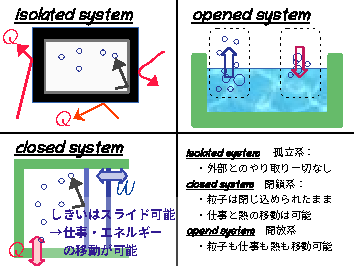
\includegraphics[keepaspectratio, width=7.5cm,height=6.9cm,clip]{neturikigaku_kankyo1.pdf}
                \caption{系の分類}
                \label{fig:neturikigaku_kankyo1}
            \end{center}
        \end{figure}

    \subsection{外界}
        着目している毛糸直接または間接的に接していて,熱や仕事,物質をやり取りする物質系を \textbf{外界} という.

    \subsection{環境}
     考察対象となる熱力学の系が置かれた周囲の状況のうち,
     室温や大気圧,熱湯(熱源)といった外界の条件をさして,これらを \textbf{環境} という.

    \subsection{拘束}
        考察対象となる熱力学の系が置かれた周囲の状況のうち,
        容器の壁やしきり,ピストンやピストンのストッパーといった,形状や体積および物質量を決める拘束条件,及び,
        断熱材や半透膜といった熱や物質の透過性を決める境界の性質,これらを \textbf{拘束} という.

    \subsection{環境と拘束}
        巨視的な系の熱平衡状態は,環境と拘束の下で,実現している.環境や拘束の変化に応じて,
        系の熱平衡状態は変化する.

    \subsection{可逆変化・非可逆変化}
        状態変化させた後で,対象とする系とその外界も含めてもとの状態に戻せる変化のこと
        を \textbf{可逆変化} という.系だけがもとに戻っ多としても,可逆変化とはいわない.
        逆に,状態を戻せない変化のことは,\textbf{非可逆変化} という.

    \subsection{断熱環境:断熱ポットの中の熱湯}
        ポットの内部には,水蒸気と空気の混合系(気体)と水の単一系(液体)の2つの部分系からなっている.
        それぞれの部分系は均質である.ポットは閉じていて,形状が固定されていることから,系の物質量と体積は
        一定に保たれている.系は熱を通さない材質の壁(\textbf{断熱壁})で囲まれていて,ポットの外部の大気の
        熱のやり取りができない.そのため,系の温度は外部の温度に影響されずに,一定の温度に保たれている.
        一方,2つの部分系(水と水蒸気・空気)の間には仕切りがなく,熱や物質を自由にやり取りできる.

        断熱ポット全体を見れば,孤立系である.内部の水と水蒸気と空気に着目すると,相互に粒子やエネルギーの
        やり取りが行えるため,個々の水と水蒸気は開放系である.
        \begin{figure}[hbt]
            \begin{center}
                \includegraphicsdefault{neturikigaku_danetu_pot.pdf}
                \caption{断熱ポット}
                \label{fig:neturikigaku_danetu_pot}
            \end{center}
        \end{figure}

    \subsection{透熱環境:シリンジの中に封入された気体}
        シリンジの内部は均質な気体の系である.ピストンとゴム栓で閉じていることで,気体の物質量は一定に保たれている.
        ピストンが\textbf{可動}である場合,内部の気体は膨張あるいは収縮ができて,体積は変化する.ピストンをストッパー
        で固定する場合は,気体の体積を一定にする拘束が加わる.系の熱を通す材質の壁(\textbf{透熱壁}:シリンジとピストン)
        で囲まれており,内部の気体はシリンジの外部の大気と熱のやりとりができる.そのため,系の温度はシリンジの外部の
        温度と等しくなる.シリンジの外部の温度・圧力は,室温・大気圧に保たれている.
        \begin{figure}[hbt]
            \begin{center}
                \includegraphicslarge{netsurikigaku_toukaheki.pdf}
                \caption{透熱壁}
                \label{fig:netsurikigaku_toukaheki}
            \end{center}
        \end{figure}

    \subsection{熱源:浴槽ないの大量の熱湯の中に置かれた鉄球}
        十分多い量の熱湯の中に小さな手球をいれた系を考える.
        熱湯と鉄球は,それぞれ均質な部分系である.鉄球は変形したり傷がついたりしないものとすれば,
        この部分の体積・物理量は一定に拘束されている.熱湯は蒸発することができ,膨張することもできる
        ので,この部分系の体積と物質量に拘束はない.鉄球と熱湯は直接的に接しているため,熱のやりとりが
        あり,その結果,どちらも温度が変わる.

        熱湯の量が十分に多く,鉄球との熱のやりとりによる温度変化が認められないとき,お湯は鉄球に対して熱の
        供給源とみなせる.これを \textbf{熱源}(\textbf{熱浴})という.ただし,大気と熱のやりとりによって
        お湯は冷めていく.一定の熱の供給源として用いるためには,湯沸かし器などによって,お湯の温度を一定に
        保つ必要がある.
        \begin{figure}[hbt]
            \begin{center}
                \includegraphicslarge{netsurikigaku_netugen.pdf}
                \caption{熱源/熱浴}
                \label{fig:netsurikigaku_netugen}
            \end{center}
        \end{figure}


    \subsection{半透膜:半透膜でしきられた希薄溶液}
    ある液体に少量の物質を溶かして作った溶液を \textbf{希薄溶液} という.溶けている物質を \textbf{溶質} といい,
    溶かすために用いる液体を \textbf{溶媒} という.また,溶媒は透過するが溶質は透過しないような膜状の物質を \textbf{半透膜} という.

    ビーカー内を半透膜で2つに仕切り,片方には溶媒のみを,もう片方には溶質と溶媒を入れる.十分時間が経過した後,ビーカー内の気迫溶液の系は,
    半透膜で仕切られた溶媒と溶質の混合系と,溶媒のみ系の2つの均質な系からなる.溶質の物質量は半透膜によって片側の系(混合系)に拘束されている.
    溶質の物質量は2つの系の間で自由にやりとりができる.

    ビーカー内の希薄溶液とビーカー外の大気との境界にしきりはなく,熱や物質を自由にやり取りできる.外界の条件は室温で大気圧にある.
    \begin{figure}[hbt]
        \begin{center}
            \includegraphicsdefault{netsurikigaku_hantoumaku.pdf}
            \caption{半透膜}
            \label{fig:netsurikigaku_hantoumaku}
        \end{center}
    \end{figure}

\section{絶対温度(気温計による定義)}
    \subsection{熱力学第0法則}
        系Aと系Bが熱平衡状態にあり,系Aと系Cが熱平衡状態にあるならば,系BとCも熱平衡状態にある.
        これは経験則で,実験事実である.熱力学の理論体系の基礎になる事柄なので,
        このことを \textbf{熱力学第0法則} といわれることも多い.ただ,熱力学の第1法則と第2法則に
        比べると,この第0法則という表現は少し非公式の感じがする.しかし,大事な原則の1つである.
        \begin{figure}[hbt]
            \begin{center}
                \includegraphicsdefault{netsu_heikou_law0.pdf}
                \caption{熱平衡(\textbf{熱力学第0法則})}
                \label{fig:netsu_heikou}
            \end{center}
        \end{figure}

    \subsection{温度}
        実際,透熱壁を介して,系Bと系Cを接触させてみると,温度など状態量に変化はなく,互いに熱平衡状態に
        あることがわかる.このように,1つの系を基準にして,他の2つの系が互いに熱平衡状態にあるかどうかを,
        直接接触させることなく判断できる.この熱平衡状態の性質は,\textbf{温度計} によって温度を定めることの
        できる原理的な理由になっている.系Aを温度計とみなせば,系Bと系Cは等しい温度にあるとえる.
        \begin{figure}[hbt]
            \begin{center}
                \includegraphicslarge{netsurikigaku_ondokei.pdf}
                \caption{温度計}
                \label{fig:netsurikigaku_ondokei}
            \end{center}
        \end{figure}

        温度の目盛りを決めるには,一般に,温度計に用いる物質の熱膨張の性質を利用する.
        ほとんどの物質は温度が高くなると体積が膨張し,温度が低くなると収縮する性質を持つ.
        熱膨張とは,温度による体積の膨張のことのことである.

        温度計に用いる物質は何でも良い.昔は(昭和,平成初期),実用的には水銀やアルコールが使われていた.
        水の凝固点(0[\circC])のときの物質の体積を${V}_{0}=$,また,
        水の沸点(100[\circC])のときの物質の体積${V}_{100}=$として,
        その差${V}_{100}-{V}_{0}$を100等分して目盛りを作る.
        このように考えた場合,温度$t$体積$V$の関数として現すことができて($t=t(V)$),
        \begin{equation}
            t(V) := 100 \times \frac{V-{V}_{0}}{{V}_{100}-{V}_{0}}
        \end{equation}
        とかける.
        逆に,温度が分かれば,体積もわかる.

    \subsection{絶対温度}
        気体は,十分に希薄でれば,その体積の膨張率は一定とみなせる.
        \begin{align}
            V &= {V}_{0} + \frac{{V}_{0}}{273.15}t  \notag \\
              &= {V}_{0}\left( 1 + \frac{1}{273.15}t \right) \notag \\
              &= {V}_{0}\left(  \frac{273.15 + t}{273.15} \right)
        \end{align}
        シャルルの法則の一例である.

        ここで,
        \begin{equation}
            T := 273.15 + t
        \end{equation}
        となる温度を新たに定義する.これを \textbf{気体温度計による絶対温度} という.すると,
        \begin{equation}
            V(T) = {V}_{0} \frac{T}{273.15} = \frac{{V}_{0}}{273.15}T
        \end{equation}
        となり,単純な比例の式になった.



%===================================================================================================
%  Chapter : 気体の状態方程式
%  説明    : ボイルの法則,シャルルの法則から,気体の状態方程式を導く
%===================================================================================================
\chapter{気体の状態方程式}
%   %-----------------------------------------------------------------------------------------------
%   %  Input
%   %    File Name : PhysNote_ST_StatGasEq.tex
%   %    説明      : 気体の状態方程式を導く
%   %-----------------------------------------------------------------------------------------------
        %       %======================================================================
%       %  Section
%       %======================================================================
        \section{ボイルの法則}
            近代科学の先駆者としてコペルニクス
                \footnote{
                    Nicolaus Copernicus (1473--1543,?):地動説を唱えたことで有名.
                    地球は太陽を中心に公転しているのだ.
                }
            やガリレイがよく挙げられる.
            それ以前には,思考のみによって世界の真理を追求してきたのだが,
            彼らは,これに疑問を訴え,観察や実験を通した事実を基に,世界の真理を
            追求すべきだと主張した.

            ボイル
                \footnote{
                    Robert Boyle (1627--1691,イギリス):化学者,物理学者.
                }
            もその考えに基づき, \textbf{自然を実験と観察に基づいて考える} という理念の下で,
            主に化学現象に関する研究を行っていた.
            その中で,ボイルは気体に関する法則を
            実験的に見出した.\textbf{ボイルの法則} である.
                \begin{myshadebox}{ボイルの法則}
                    温度を一定に保っている状態では,圧力と体積は反比例の関係にある.
                    言い換えると,圧力と体積の積は一定値を保つ.
                    圧力を $p$,体積を $V$ としたとき,
                    \begin{align}
                        pV = k. \mbox{(温度一定)}
                    \end{align}
                    ここで,$k$ は気体の初期状態により決まる定数.
                \end{myshadebox}

            ボイルの法則や,この後に説明するシャルルの法則は,熱力学の教科書だけでなく,
            化学の教科書にも登場する.その意味で,熱力学と化学を結ぶ重要な法則である.


%       %======================================================================
%       %  Section
%       %======================================================================
        \section{シャルルの法則}
            シャルル
                \footnote{
                    Jacques Alexandre C\'{e}sar Charles (1746--1823):化学者.
                }
            気体に関する法則を実験的に見出した.\textbf{シャルルの法則} とよばれる.
                \begin{myshadebox}{シャルルの法則}
                    圧力を一定に保っている状態では,体積と温度は比例関係にある.
                    言い換えると,体積と温度の比は一定値を保つ.
                    体積を $V$,温度を $T$ としたとき,
                    \begin{align}
                        \frac{V}{T} = l. \mbox{(圧力一定)}
                    \end{align}
                    ここで,$l$ は気体の初期状態により決まる定数.
                \end{myshadebox}

            比例定数についても実験的に得られる.もう少しシャルルの法則を詳しく書くと,
            次よようになる.すなわち,\textbf{一定圧力において,気体の体積は,
            温度を1度上昇させると,0度の時の体積の1/273ずつ増加する}.
            式で表すと,0度の時の体積を ${V}_{0}$ とし,温度t度上昇させた時の,気体の体積 $V(t)$ は,
                \begin{equation*}
                    V(t) = \frac{1}{273} {V}_{0}t + {V}_{0}.
                \end{equation*}
            次のように式変形してみよう.
                \begin{equation*}
                    V(t) = \left( \frac{1}{273}t + 1 \right) {V}_{0} = \frac{t+273}{273} {V}_{0}.
                \end{equation*}
            $T=t+273$ を導入して,
                \begin{equation*}
                    V(t) = \frac{T}{273} {V}_{0}
                \end{equation*}
            となる.この $T$ のことを \textbf{絶対温度} といい,単位を [K] で表す.
            [K] は「ケルビン」と読む.
                \begin{figure}[hbt]
                    \begin{center}
                        \includegraphicsdefault{charlesNohousoku.pdf}
                        \caption{シャルルの法則}
                        \label{fig:charlesNohousoku}
                    \end{center}
                \end{figure}


%       %======================================================================
%       %  Section
%       %======================================================================
        \section{ボイル$=$シャルルの法則}
            ボイルの法則とシャルルの法則を1つにまとめることができる.
            ひとまとめにできることを示すには,実際に状態遷移の計算をしてみて,
            矛盾がないことを確認すればいい.

            温度 $T$ と体積 $V$ と圧力 $p$ の添字のアルファベット(A, B, C)は,
            図\ref{fig:BoyleCharlesTotal1111}で示す状態に対応する.
            状態遷移は次のように行う.まず,最初の状態をAとする.状態Aから
            等温変化させて,状態Bへ移す.この時,等温変化であるから,ボイルの
            法則が成り立つはずである.更に,状態Bから状態Cへ等圧変化により
            遷移させる.この場合は,等圧変化であるので,シャルルの法則が
            成り立つはずである.最後に,状態Aと状態Cにおける各温度,体積,圧力
            の関係が等しければ,ボイルの法則とシャルルの法則をひとまとめに
            できることが示される.
            \begin{figure}[hbt]
                \begin{center}
                    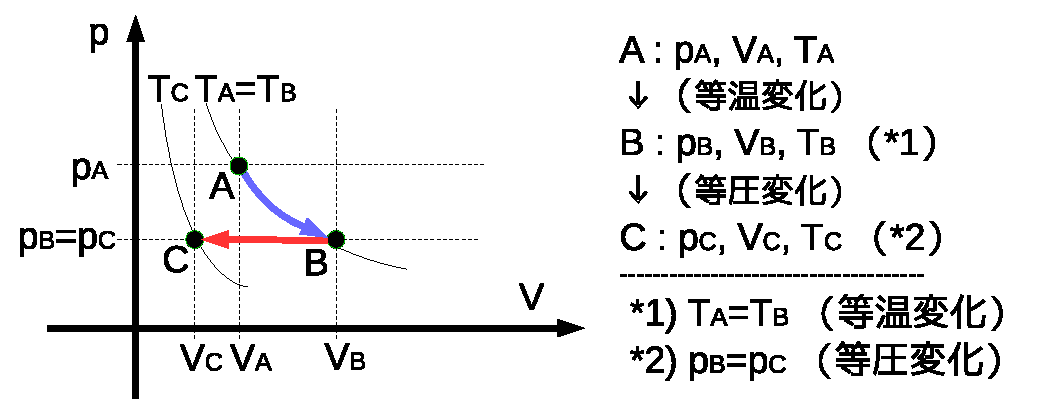
\includegraphics[keepaspectratio, width=8.0cm,height=3.3cm,clip]{BoyleCharlesTotal1111.pdf}
                    \caption{ボイル$=$シャルルの法則}
                    \label{fig:BoyleCharlesTotal1111}
                \end{center}
            \end{figure}

            一定温度 $T_{A}$ の下で,ボイルの法則により,
                \begin{equation*}
                    {p}_{A}{V}_{A} = {p}_{B}{V}_{B}.
                \end{equation*}
            後の式変形のため,${V}_{B}$ について解いておく.
                \begin{equation*}
                    {V}_{B} = \frac{{p}_{A}{V}_{A}}{{p}_{B}}.
                \end{equation*}

            引き続き,一定圧力 $p_{B}$ の下で,シャルルの法則より,
                \begin{equation*}
                    \frac{{V}_{B}}{{T}_{B}} = \frac{{V}_{C}}{{T}_{C}}.
                \end{equation*}
            ${V}_{B}$ を置き換えて,
                \begin{equation*}
                    \frac{{p}_{A}{V}_{A}}{{T}_{B}{p}_{B}} = \frac{{V}_{C}}{{T}_{C}}.
                \end{equation*}
            両辺に ${p}_{B}$ をかけておく.
                \begin{equation*}
                    \frac{{p}_{A}{V}_{A}}{{T}_{B}} = \frac{{p}_{B}{V}_{C}}{{T}_{C}}.
                \end{equation*}

            ここで,状態AからBの遷移は等温変化であるので,
                \begin{equation*}
                    {T}_{B} = {T}_{A}.
                \end{equation*}
            また,状態Bから状態Cへの遷移は等圧変化であるので,
                \begin{equation*}
                    {p}_{B} = {p}_{C}.
                \end{equation*}
            この2点を考慮すると
                \begin{equation*}
                    \frac{{p}_{A}{V}_{A}}{{T}_{A}} = \frac{{p}_{C}{V}_{C}}{{T}_{C}}.
                \end{equation*}
            式の添字に着目すれば,最初の状態Aと最後の状態Cにおいて,
            関係式 $pV/T$ が同じ値をとることがわかる.この値を $k$ と書くことにすれば
                \footnote{
                    \begin{equation*}
                        k := \frac{{p}_{A}{V}_{A}}{{T}_{A}} = \frac{{p}_{C}{V}_{C}}{{T}_{C}}.
                    \end{equation*}
                },
                \begin{equation*}
                    \frac{pV}{T} = k.
                \end{equation*}
            次のように書き換えれば,よく見かける方程式になる.
                \begin{equation*}
                    pV=kT.
                \end{equation*}
            これが,\textbf{ボイル$=$シャルルの法則} である.
            ボイル$=$シャルルの法則の式は,\textbf{気体の状態方程式} とよばれる.

            まとめておこう.
                \begin{myshadebox}{ボイル$=$シャルルの法則}
                    気体において,温度 $T$,体積 $V$,圧力 $p$ は,
                    定数 $k$ を用いて,以下の関係式を満たす.
                    \begin{align}
                        pV=kT.
                    \end{align}
                \end{myshadebox}

%       %======================================================================
%       %  Section
%       %======================================================================
        \section{理想気体}
        理想気体の状態方程式が厳密に成り立つ理想的な気体のことを \textbf{理想気体} という.
        理想気体は実在しないが,高温状態あるいは低圧状態では,実在する気体を理想気体と
        みなしうることができる,ということもある.実際は,工学的には,理想と現実の乖離具合
        を常に意識しなければならない.ただ,理論構築のためには,理想気体はとても
        有用なので,熱力学では理想気体が主役になる.理想気体の性質を理論的に把握することで,
        現実に存在する \textbf{実在気体} の性質を推察できるようになる.
        どれだけ実在気体が理想気体と乖離しているかが,実在気体の特徴であるともいえる.

%       %======================================================================
%       %  Section
%       %======================================================================
        \section{状態方程式}
        \begin{mycomment}
            気体が従う自然法則(方程式)を導入する.
            熱力学では,ニュートンの運動方程式と同じように,天下り的に与えられる式であり,他から導き出されるものではない.
            気体を無数の粒子の集まりとして仮定した統計力学から,理想気体の状態方程式を導けるが,これは熱力学の論理の範囲外である.
            今は熱力学を学習しているため,状態方程式は実験事実の自然法則として受け入れよう.
        \end{mycomment}
        \subsection{理想気体の状態方程式}
        状態方程式は熱力学の基本法則の1つである.以下に書き下そう.
        \begin{myshadebox}{理想気体の状態方程式}
            理想気体において,圧力$P$[N/m${}^{2}$],体積$V$[m${}^{3}$],物質量$n$[mol], 温度$T$[K],
            気体定数$R$[J/mol$\cdot$K]の条件下で,以下が成り立つ.
            \begin{equation}
                PV = nRT.
            \end{equation}
        \end{myshadebox}

        理想気体の状態方程式のことは,混乱の恐れがない場合には,単に,状態方程式ともいう.

        \subsection{気体の濃度}
        体積$V$[m${}^{3}$]の容器の中に$n$[mol]の気体が入っているとき,この気体の濃さを
        数値化できる.同じ堆積中で,たくさん気体が入っていれば濃くなるし,少なければ,
        薄くなる.これを \textbf{濃度} という.濃度を$\sigma$で現すと,
            \begin{align}
                \sigma = \frac{n}{V}
            \end{align}
        である.状態方程式と対比させてみと,以下になる.
            \begin{align*}
                 PV &= nRT \\
                \Leftrightarrow P &= \frac{n}{V}RT \\
                \Leftrightarrow P &= \sigma RT \\
            \end{align*}

        濃度$\sigma = n/V$が一定の場合に成立する式だ.圧力は濃度に比例する.
        気体の濃度が濃いほど圧力は高くなるのだ.
        \begin{align}
            P(T) = \sigma RT.
        \end{align}

        注意すべきは式を濃度$\sigma$について解いてみて
        \begin{align}
            \sigma = \frac{P}{RT}
        \end{align}
        としてしまうと,あたかも濃度が圧力に比例するようにみえる.この解釈は間違いである.
        濃度はもともと,$n/V$であることを忘れてはいけない.$n$の値は変化しない(急に気体が湧いて出たりしない).
        つまり,圧力が変化して濃度が変わったのであれば,実際には体積$V$が変化したということである.
        圧力$P$を高くして体積$V$をぐぐっと縮みることで,濃度が高くなるのだ.

        \subsection{実在気体の状態方程式}
        \subsubsection{ビリアル方程式}
        \subsubsection{ファンデルワールスの状態方程式}
        実在する気体の振る舞いをいい感じに表現する方程式がある.液体にも適用可能である.
        ファンデルワールス
            \footnote{
                Johannes Diderik van der Waals(1837--1923,オランダ):ヨハネス ディーデリク ファン デル ワールス.
                1910年にこの気体の状態方程式の発見によりノーベル賞を受賞している.分子間力の1つである,
                \textbf{ファンデルワールス力}(\textbf{ファンデルワールス結合})でもその名前が知られている.
            }というオランダ人の物理学者が提案した,実在気体の状態方程式である.
        気体の種類によって,振る舞いが異なるので,それに対応する特徴的な 定数$a$,$b$が使われる.

        ファンデルワールスの状態方程式も他から導かれるものではないが,雰囲気からなら説明・導入ができる.
        理想気体の状態方程式に現実的要素を織り交ぜて,変形していく.理想気体からの乖離を補正するのである.
        補正を受けるのは,体積$V$と圧力$P$である.まず,体積から考えよう.

        理想気体を構成する粒子は体積はないものと仮定されていた
            \footnote{
                実際,熱力学が成立した時代にも,原子や分子の存在は知られていなかった.
                確かに,デモクリトストスが提唱していたと言われているが,空想上の概念であり,
                デモクリトスが実験的に原子や分子の存在を確かめたわけではない.
            }.
        しかし,実在気体を構成する粒子は,一つ一つは微小であるが,体積を持つ.
        現実気体$n$[mol]の体積を${V}_{R}$(RealのR),おなじく理想気体$n$[mol]の体積を${V}_{I}$(ImageのI)とするならば,
        体積の補正項を$b$を導入して,
            \begin{equation}
                {V}_{R} = {V}_{I} + bn
            \end{equation}
        と書ける.実在気体の体積は理想気体の体積よりも,粒子自体の大きさ分だけ,大きいと考える.
        \begin{figure}[hbt]
            \begin{center}
                \includegraphicsmiddle{netsurikigaku_van_der_waals_force.pdf}
                \caption{実在気体:体積}
                \label{fig:netsurikigaku_van_der_waals_force}
            \end{center}
        \end{figure}

        実在の気体の圧力も理想とは異なる.実際には分子を構成する原子機構により分子内部の電子の位置が偏り,
        分子自体に正負の電気的な偏りができる.これが複数存在すると,分子のプラス側(正)と別の分子のマイナス側(負)が
        引き合う現象がおきる.これを \textbf{分子間力} という
            \footnote{
                分子間力といっても,発生機構によって細分化される.イオン間相互作用,水素結合,双極子相互作用,ファンデルワールス力.
            }.
        分子間力が働くと,分子の運動が束縛されて(分子の運動が鈍くなり),結果,圧力が弱まる.
        \begin{figure}[hbt]
            \begin{center}
                \includegraphicsmiddle{netsurikigaku_van_der_waals_force2.pdf}
                \caption{実在気体:圧力}
                \label{fig:netsurikigaku_van_der_waals_force2}
            \end{center}
        \end{figure}
        では,どの程度弱まるのか.モル濃度の2乗に比例すると考えられている(根拠は実験かな).
        現実気体$n$[mol]の圧力を${P}_{R}$(RealのR),おなじく理想気体$n$[mol]の圧力を${P}_{I}$(ImageのI)とするならば,
        圧力の補正項を$a$を導入して,
        \begin{equation}
            {P}_{R} = {P}_{I} - a{\left( \frac{n}{{V}_{I}} \right)}^{2}
        \end{equation}
        となる.

        理想気体の状態方程式は厳密に成り立つ.${V}_{I}$と${P}_{I}$を使って理想気体の状態方程式を書くならば,
        \[
            {P}_{I}{V}_{I} = nRT.
        \]
        だけど,${V}_{I}$と${P}_{I}$は実在気体の体積と圧力だから,この式は間違っている.式を補正して正しくしよう.
        この理想気体型の状態方程式に,さっき計算した結果を適用すればよい.
        まず,上記の2つの式をそれぞれ,${V}_{I}$と${P}_{I}$について解くと,
        \begin{align}
            {V}_{I} &= {V}_{R} - bn \\
            {P}_{I} &= {P}_{R} + a{\left( \frac{n}{{V}_{I}} \right)}^{2}
        \end{align}
        である.これを状態方程式に代入しよう.
        \begin{equation}
            \left( {P}_{I} + a{\left( \frac{n}{{V}_{I}} \right)}^{2} \right) \left( {V}_{I} - bn \right) = nRT.
        \end{equation}
        カッコが多くてきたないので,適当に外すと,
        \begin{equation}
            \left( {P}_{I} + a\frac{{n}^{2}}{{{V}_{I}}^{2}} \right) \left( {V}_{I} - bn \right) = nRT.
        \end{equation}
        となる.

        これを \textbf{ファンデルワールスの状態方程式} という.
        また,$a$,$b$のことを \textbf{ファンデルワールス定数} という.
        \begin{myshadebox}{ファンデルワールスの状態方程式}
            現実気体$n$[mol]の圧力を${P}_{I}$,現実気体$n$[mol]の体積を${V}_{I}$として(RealのR),
            \begin{equation}
                \left( {P}_{I} + a\frac{{n}^{2}}{{{V}_{I}}^{2}} \right) \left( {V}_{I} - bn \right) = nRT.
            \end{equation}
        \end{myshadebox}

        「理想気体の圧力に対して,実在気体の圧力は分子間力の分だけ小さくなるので,補正項を足す」,
        「理想気体の体積に対して,実在気体の体積は大きさがある分だけ大きくなるので,補正項を引く」
        と捉えておけばよいだろう.

        ちなみに,教科書には${P}_{I}$を左辺にした表現となっていた.
        \begin{equation}
             {P}_{I}  =  \frac{nRT}{\left( {V}_{I} - bn \right)} - a{\left(\frac{n}{{V}_{I}} \right)}^{2}.
        \end{equation}
        ちょっと細工すると,
        \begin{equation*}
            {P}_{I}  =  \frac{1}{\left( {V}_{I} - bn \right)}nRT - a{\left(\frac{n}{{V}_{I}} \right)}^{2}.
       \end{equation*}
        この表現からは,現実気体の圧力は,理想気体の$1/({V}_{I} - bn)$で,さらに,分子間力がはたらく分だけ
        小さくなることが読み取りやすい.

%       %======================================================================
%       %  Section
%       %======================================================================
        \section{分圧の法則}
        混合気体が入った容積の圧力を考える.この容積内部の圧力について,以下の法則が成り立っている.
        \begin{myshadebox}{分圧の法則}
            混合気体の圧力(全圧)は,それを構成する各々の種類の成分圧力(分圧)
            の和に等しい.気体は何種類もあってよくて,$k$種類の気体がある場合は
            以下の式が成り立つ.
            \begin{equation}
                P = \sum_{i=1}^{k} {p}_{i}
            \end{equation}
            左辺の$P$が全圧であり,右辺の${p}_{i}$($i=1,\,2,\,\cdots,\,n$)が分圧である.
        \end{myshadebox}
        ドルトンが提唱した法則なので,「ドルトンの分圧の法則」とかと紹介されることも多い.

        \begin{figure}[hbt]
            \begin{center}
                \includegraphicsmiddle{netsurikigaku_bunsi_undo_ron_bunatsu.pdf}
                \caption{全圧と分圧}
                \label{fig:netsurikigaku_bunsi_undo_ron_bunatsu}
            \end{center}
        \end{figure}

        う〜ん,この法則はどうやって実験的に確かめたのだろうか.
        原理的には,こうだろう.まず,同体積の気体A,B,Cを用意して,
        それぞれの圧力の計測する.これは,後で気体を混合した場合に,元々の各気体の分圧の測定とみなせる.
        その結果をそれぞれ${P}_{A}$,${P}_{B}$,${P}_{C}$であったとしよう.
        次に,同じ体積ににA,B,Cの3つの気体を同じ一つの箱に押し込めて,圧力を測定する.
        たとえば,BとCをAの箱に詰めるなど.そうすると,3種類の全気体が1箇所に集まることになり,
        このAとBとCから構成される全気体の圧力(すなわち全圧)の測定が可能になる.
        分圧の法則にしたがえば,全圧を単に$P$すると,
            \[
                P = {P}_{A} + {P}_{B} + {P}_{C}
            \]
        と計算できる.

        気体が分子から構成されていることと理想気体の状態方程式から,分圧の法則が導けないだろうか.
        もう少し遊んでみよう.
        
        状態方程式$PV=nRT$から,$P=(n/V)RT$.温度$T$は一定であるとする.すると,
        \[
            \frac{n}{V}RT = \frac{{n}_{A}}{{V}_{A}}RT + \frac{{n}_{B}}{{V}_{B}}RT + \frac{{n}_{C}}{{V}_{A}}RT.
        \]
        ${n}_{A}$,${n}_{B}$,${n}_{C}$はA,B,Cのそれぞれのモル数.
        ${V}_{A}$,${V}_{B}$,${V}_{C}$はそれぞれ,A,B,Cの体積である.体積は同じで,
        \[
            V = {V}_{A} = {V}_{B} = {V}_{C}.
        \]
        だから,
        \begin{align*}
            \frac{n}{V}RT &= \frac{{n}_{A}}{V}RT + \frac{{n}_{B}}{V}RT + \frac{{n}_{C}}{V}RT.
        \end{align*}
        気体の単位体積あたりのモル数(濃度)$\sigma$を考えて,
        \[
            {\sigma}     :=\frac{n}{V},       \quad {\sigma}_{A} :=\frac{{n}_{A}}{V}, \quad
            {\sigma}_{B} :=\frac{{n}_{B}}{V}, \quad {\sigma}_{C} :=\frac{{n}_{C}}{V}
        \]
        と書くことにすると,
        \begin{align*}
                            {\sigma} RT &= {\sigma}_{A} RT + {\sigma}_{B} RT + {\sigma}_{C} RT \\
            \Leftrightarrow {\sigma}    &= {\sigma}_{A}    + {\sigma}_{B}    + {\sigma}_{C}.
        \end{align*}
        となる.体積が一定であれば,それぞれの気体を混ぜ合わせた後の濃度は,それぞれの
        濃度の足し算で計算できる.体積$V$がみえるようにかくと,
        \begin{align*}
                          {\sigma} &= {\sigma}_{A}     + {\sigma}_{B}      + {\sigma}_{C} \\
                       \frac{n}{V} &= \frac{{n}_{A}}{V} + \frac{{n}_{B}}{V} + \frac{{n}_{C}}{V} \\
            \therefore           n &= {n}_{A} + {n}_{B} + {n}_{C}
        \end{align*}
        である.容積中の全体の気体のモル数は,個々の気体のそれぞれのモル数を足し合わせたものである.

        このモル数の足し合わせの結果をベースにして,温度と体積が一定であるという条件の下で,
        これまでの議論を逆にたどれば,分圧の法則が導ける.
        \begin{align*}
                                        n &= \sum_{i=1}^{k} {n}_{i}\\
            \Leftrightarrow \frac{n}{V}   &= \frac{1}{V}\sum_{i=1}^{k} {n}_{i} = \sum_{i=1}^{k} \frac{{n}_{i}}{V}\\
            \Leftrightarrow \frac{n}{V} T &= \left(\sum_{i=1}^{k} \frac{{n}_{i}}{V}\right)  T = \sum_{i=1}^{k}\left( \frac{{n}_{i}}{V} T\right)\\
            \Leftrightarrow \frac{n}{V}RT &= \left(\sum_{i=1}^{k} \frac{{n}_{i}}{V}\right) RT= \sum_{i=1}^{k}\left( \frac{{n}_{i}}{V}RT\right)  \\
            \Leftrightarrow             P &= \sum_{i=1}^{k} {p}_{i}.\quad\mbox{(分圧の法則が導けた)}\
        \end{align*}
        どちらかと言うと,モル数をベースにしたほうが直感的で理解しやすいと思う.ただ,式変形に物理的な洞察はなく,説得力に欠ける.
        モル数をベースにして,温度と圧力が一定だったら,必然的に,分圧の法則が成り立つ,という事実が説明できるだけだ.





\chapter{気体分子運動論}
%   %-----------------------------------------------------------------------------------------------
%   %  Input
%   %    File Name : PhysNote_GasMolTheory.tex
%   %    説明      : 気体分子運動論を学習する.気体は多数の微粒子の集まりとして考える
%   %-----------------------------------------------------------------------------------------------
        %   %==========================================================================
%   %  Comment
%   %==========================================================================
\begin{mycomment}
    気体についての考察.気体は無数の分子から構成されていると言う仮定して,
    気体の圧力や分子の運動エネルギーについて調べてみよう.
\end{mycomment}

\section{仮定}
    気体分子運動論を考える状況について,議論の最初に,いくつか仮定を設けておく.
    \begin{itembox}[l]{気体分子運動論の仮定}
        \begin{itemize}
            \item 気体は理想気体を対象とし,分子間力は考えない
            \item 分子は数え切れないほど多く存在し,巨視的に見れば,
                  あらゆる方向に均一に運動している($x$,$y$,$z$の全方向に均一である)
            \item 分子同士の衝突はないものとする(衝突しても結果は変わらないが,状況が複雑になり計算が面倒になる)
            \item 分子と壁は弾性衝突する(衝突係数$=1$:跳ね返りによるエネルギーの散逸なし)
            \item 重力の影響はないものとする
            \item 1辺が$L$[m]の立方体の容器に入った気体分子を考える(体積は$V={L}^{3}$[m${}^{3}$])
        \end{itemize}
    \end{itembox}

\section{分子の速度とその平均}
    まず,立方体のある1つの分子に着目する.
    この分子の速度を$\bv$とする.速度は3次元であるので,$\bv$は$x$,$y$,$z$成分に分解できる.
    \begin{equation}
        \bv = ({v}_{x},\,{v}_{y},\,{v}_{z}).
    \end{equation}
    他のベクトル量も3次元であり,速度と同様に3つの成分を持つ.
    後で使うので,速度の2乗平均$\bar{{v}^{2}}$も計算しておこう.

    まず,速度ベクトルを2乗する.
    \[
        {\bv}^{2} = {v}^{2} = {{v}_{x}}^{2} + {{v}_{y}}^{2} + {{v}_{z}}^{2}
    \]
    すべての分子の平均をかんがえると,
    \begin{align*}
        \bar{{\bv}^{2}} &= \bar{{v}^{2}} \\
                        &= \bar{{{v}_{x}}^{2} + {{v}_{y}}^{2} + {{v}_{z}}^{2}} \\
                        &= \bar{{{v}_{x}}^{2}} + \bar{{{v}_{y}}^{2}} + \bar{{{v}_{z}}^{2}}
    \end{align*}
    さらに,あらゆる方向に均一に運動しているので,
    \[
        \bar{{{v}_{x}}^{2}} = \bar{{{v}_{y}}^{2}} = \bar{{{v}_{z}}^{2}}
    \]
    としてよい.一旦${v}_{x}$だけの式にする.
    \[
        \bar{{v}^{2}} = 3\bar{{{v}_{x}}^{2}}
    \]
    これより,
    \begin{equation}
        \bar{{{v}_{x}}^{2}} = \frac{1}{3} \bar{{v}^{2}}
    \end{equation}
    を得る.この速度の式は後の計算で使うことになる.

    \begin{memo}{$N$個の分子の速度の2乗平均}
        この部分の計算で,現れた速度の2乗平均の計算方法を確認しておこう.
        $N$個の分子に,1から$N$の自然数で番号付けをしておこう.そして,
        $N$個の各々の分子の速度を,${v}_{i}$としよう.添字の$i$は1から$N$までの
        いずれかの自然数である.自然数$i$をきめると,対応する分子が定まるこのとになる.
        平均とは全部(ここでは$N$個)のデータを合計して,その総数(ここでは$N$個)で割った
        値のことである.${v}_{1}$,${v}_{2}$,${v}_{3}$,$\cdots$ の値はそれぞれ異なる.
        個々の値には興味はなく,その平均が知りたい.ここで知りたいのは速度の大きさの
        平均である.速度は正負の向きを持ったベクトルなので,このまま足し合わせても
        速さの平均値を求めることはできない
            \footnote{
                極端な例を上げよう.速度には正負の向きがあるため,
                たまたま,すべてを合計したら0になるかのせいもある.
                平均の速度が0となる.ベクトルとしてはそれで正解であるが,
                速さの平均を求めたいのであるから,平均が0になっていしまうのは困る.
                各々の絶対値をとる方法も考えれるかもしれないが,二乗して必ず正の値に
                なるように細工したほうが都合が計算しやすいし,式も見やすいし良い.
                二乗しているので,計算の最終段階で平方根を求めれば良い.
            }.
        そこで,速度の2乗平均を計算することにしよう.実は,運動エネルギーも速度の
        2乗でであるため,この方法が都合が良い.

        すると,速度の2乗平均は以下のように計算される.
        \begin{align*}
            \bar{{\bv}^{2}} &= \frac{1}{N} \left( {{\bv}_{1}}^{2} + {{\bv}_{2}}^{2} + \cdots + {{\bv}_{N}}^{2} \right ) \\
                            &= \frac{1}{N} \sum_{i=1}^{N} {{\bv}_{i}}^{2}.
        \end{align*}

        速さが知りたかったら,平方根取ればいい.
        \[
            v = \sqrt{\bar{{\bv}^{2}}} = \sqrt{\frac{1}{N} \sum_{i=1}^{N} {{\bv}_{i}}^{2}}.
        \]
    \end{memo}

    \section{分子1つが壁に衝突するときに,壁に与える平均の力:$\bar{{f}_{x}}$}
    まずは$x$軸方向のみを考えよう.
    \begin{figure}[hbt]
        \begin{center}
            \includegraphicslarge{netsurikigaku_bunsi_undo_ron.pdf}
            \caption{気体分子運動論}
            \label{fig:netsurikigaku_bunsi_undo_ron}
        \end{center}
    \end{figure}

    最初に,「壁が分子から受ける力積」を計算する.この力積を${I}_{x}$とする.
    計算したいのだが,壁の速度に変化がないので,壁の運動から直接的に計算できない.
    そこで,分子と壁の作用反作用の法則を利用する.つまり,
        \[
            \mbox{分子の受ける力積} = - \mbox{壁の受ける力積}
        \]
    が成り立っているはずなので,分子の受ける力積を計算して,符号を反対にすればよい.
    力積は運動量の変化分に等しく,
        \[
            \mbox{力積} = \mbox{衝突後の運動量} - \mbox{衝突前の運動量}
        \]
    である.運動量$m{v}_{x}$で運動していた分子は壁に衝突すると,速度は反対向きになり,$m(-{v}_{x})$となる.
    また,分子が壁から受ける力積は$x$軸方向の反対なので,符号はマイナスである.
    これに当てはめると,分子が壁から受ける力積$-{I}_{x}$は
    \begin{align*}
        - {I}_{x}   &= - \bar{{f}_{x}}  t     \\
                    &= m(-{v}_{x}) - m{v}_{x} \\
                    &= -m{v}_{x} - m{v}_{x}   \\
                    &= -2m{v}_{x}
    \end{align*}
    である.$\bar{{f}_{x}}$は一回の衝突で与える$x$方向の力の大きさである.
    これより,壁が分子から受ける力積${I}_{x}$は,
    \begin{equation}
        {I}_{x} = \bar{{f}_{x}}  t = 2m{v}_{x}
    \end{equation}
    となる
        \footnote{
            ちなみに,「壁が分子から受ける力積」を言い換えれば,「分子が壁に与える力積」である.
            言葉の表現による注意も怠りなく.
        }.

    次に,「1つの分子が$t$秒間に壁に与える力積」を計算する.壁にあたった瞬間を$t=0$としたとき,
    分子は往復で$2L$の距離を速度${v}_{x}$で運動しているわけだから,次に衝突する時間を$t'$とすれば,
    \[
        2L = {v}_{x}t'
    \]
    が成立している.$t'$について解いて,
    \[
        t' = \frac{2L}{{v}_{x}}
    \]
    としておこう.分子が壁に1回衝突するのにかかる時間が$t'=2L/{v}_{x}$であることがわかった.
    であれば,$t$秒間に衝突する回数$n$は,$t/t'$を計算すればよく,
    \[
        n = \frac{t}{t'}=\frac{t}{2L/{v}_{x}}=\frac{{v}_{x}t}{2L}
    \]
    となる.
    \begin{figure}[hbt]
        \begin{center}
            \includegraphicslarge{netsurikigaku_bunsi_undo_ron2.pdf}
            \caption{壁への衝突回数}
            \label{fig:netsurikigaku_bunsi_undo_ron2}
        \end{center}
    \end{figure}

    分子が壁に与える1回あたりの力積${I}_{x}$は${I}_{x} = \bar{{f}_{x}}  t = 2m{v}_{x}$であった.これを使えば,
    $t$秒間に分子1つが壁に与える力積がわかる.以下のとおりである.
    \[
        2m{v}_{x} \times \frac{{v}_{x}t}{2L}=\frac{m{{v}_{x}}^{2}}{L}t=\bar{{f}_{x}}  t.
    \]

    したがって,最後の等式の対応見れば,壁に与える平均の力$\bar{{f}_{x}}$がわかる.
    \begin{equation}
        \bar{{f}_{x}} = \frac{m{{v}_{x}}^{2}}{L}.
    \end{equation}

    \begin{figure}[hbt]
        \begin{center}
            \includegraphicsdefault{netsurikigaku_bunsi_undo_ron_rikiseki.pdf}
            \caption{力積}
            \label{fig:netsurikigaku_bunsi_undo_ron_rikiseki}
        \end{center}
    \end{figure}

    \section{分子N個が壁に衝突するときに,壁に与える平均の力:$\bar{{F}_{x}}$}
    分子$N$個の衝突によって,壁が受ける平均の力が知りたい.これは$\bar{{f}_{x}}$を$N$倍することで
    計算できる.ただし,注意が必要である.いままでは1つの分子について着目していたため,${{v}_{x}}^{2}$は
    確かな固定値であった.しかし,今回は$N$個の分子を対象にしており,すべての分子が一律に${{v}_{x}}^{2}$という
    速度で運動しているはずがなく,このまま${{v}_{x}}^{2}$すれば,誤りとなる.ではどうするかと言うと,
    答えは簡単で,$N$個の分子の速度の平均値を考えれば良い.これを$\bar{{{v}_{x}}^{2}}$とかくことにしよう.
    \begin{equation}
        \bar{{F}_{x}} = \frac{Nm\bar{{{v}_{x}}^{2}}}{L}.
    \end{equation}


    \section{気体の圧力:$P$}
    圧力とは,単位面積あたりの力のことであった.今の場合,面積は${L}^{2}$である.
    $N$個の分子からなる気体が発生させる圧力$P$は
    \[
        P = \frac{\bar{{F}_{x}}}{{L}^{2}} = \frac{Nm\bar{{{v}_{x}}^{2}}}{L{L}^{2}} = \frac{Nm\bar{{{v}_{x}}^{2}}}{{L}^{3}}
    \]
    である.ここで,${L}^{3}$は立方体の体積であるから,$V$という文字で置き換えておこう($V:={L}^{3}$).
    \[
        P = \frac{Nm\bar{{{v}_{x}}^{2}}}{V}
    \]
    さらに,さっき計算した速度の式
    \[
        \bar{{{v}_{x}}^{2}} = \frac{1}{3} \bar{{v}^{2}}
    \]
    を適用すると,
    \[
        P = \frac{Nm \left((\frac{1}{3} \bar{{v}^{2}}\right)}{V} =\frac{Nm\bar{{v}^{2}}}{3V}.
    \]
    となる.

    \section{分子1つの並進運動エネルギーの平均値}
    理想気体の状態方程式 $PV=nRT$に関連付けたいので,両辺に$V$をかけよう.
    \[
        PV = nRT =  \frac{Nm \left(\frac{1}{3} \bar{{v}^{2}}\right)}{V} =\frac{Nm\bar{{v}^{2}}}{3}.
    \]
    分子1つの運動エネルギーは$m\bar{{v}^{2}}/2$であるから,この式から抽出してみよう.
    $m\bar{{v}^{2}}/$について解いてから,両辺に$1/2$をかけるとよいだろう.
    \begin{align*}
                                   nRT &= \frac{Nm\bar{{v}^{2}}}{3} \\
        \Leftrightarrow m\bar{{v}^{2}} &= \frac{3nRT}{N} \\
        \Leftrightarrow \frac{1}{2}m\bar{{v}^{2}} &= \frac{3}{2} \frac{n}{N}RT.
    \end{align*}
    ここで,$n/N$に注目しよう.$N$は気体分子全部の個数で,$n$は物質量([mol])である.
    つまり,$N$を$n$で割ると,1[mol]あたりの分子の個数が計算できて,これはアボガドロ定数${N}_{A}$であり,
    \[
        {N}_{A} = \frac{N}{n}
    \]
    であるから,$n/N$を$1/{N}_{A}$で置き換えられる.
    \begin{align*}
        \frac{1}{2}m\bar{{v}^{2}} &= \frac{3}{2} \frac{R}{{N}_{A}}T.
    \end{align*}
    後で詳しく学習するが,$R/{N}_{A}$はボルツマン定数${k}_{B}$であり,以下を得る.
    \begin{equation}
        \frac{1}{2}m\bar{{v}^{2}} = \frac{3}{2} {k}_{B}T.
    \end{equation}
    分子の運動エネルギーの平均値は,絶対温度$T$のみにより定まり,気体種類には依存しないことがわかる.

    \section{単原子分子からなる理想気体の内部エネルギー}
    N個の単原子分子からなる理想気体の内部エネルギー$U$は,内部の分子の運動エネルギーの平均を$N$倍すればいい.
    \begin{align*}
        U &= N \times \frac{1}{2}m\bar{{v}^{2}} \\
          &= N \times \frac{3}{2} \frac{R}{{N}_{A}}T    \\
          &= \frac{3}{2} \frac{N}{{N}_{A}}RT
    \end{align*}
    ここで,$n=N/{N}_{A}$だから,
    \begin{equation}
        U = \frac{3}{2} nRT = \frac{3}{2} PV.
    \end{equation}
    単原子分子の内部エネルギーは絶対温度で定まり,絶対温度に比例する.

    考えなければならず,この結果は多原子分子には適用できない.
    \begin{figure}[hbt]
        \begin{center}
            \includegraphicslarge{netsurikigaku_bunsi_undo_ron_tangensibunsi.pdf}
            \caption{多原子分子の場合は回転の考慮も必要}
            \label{fig:netsurikigaku_bunsi_undo_ron_tangensibunsi}
        \end{center}
    \end{figure}
